\documentclass[xcolor=svgnames,compress]{beamer}

% see http://tex.stackexchange.com/questions/13423/how-to-color-href-links-in-beamer
\hypersetup{colorlinks,linkcolor=,urlcolor=DarkGreen}

\mode<presentation>
{
  \usetheme{Warsaw}
  \setbeamertemplate{navigation symbols}{}
  \setbeamercovered{dynamic}
}

\usepackage[spanish,es-noshorthands]{babel}
\usepackage[utf8x]{inputenc}
\usepackage[T1]{fontenc}
\usepackage{csquotes}
\usepackage{tikz}
\usepackage{fancyvrb}
\usepackage[htt]{hyphenat}
\usepackage{array}
\usepackage{marvosym}
\PrerenderUnicode{áéíóúÁÉÍÓÚçÇ}

\usepackage{pgfplots}
\pgfplotsset{compat=1.3}
% Taken from jake's comment on
% http://tex.stackexchange.com/questions/3983. Thanks!
%
% SAMPLE CODE
%
% \begin{filecontents}{testdata.dat}
% 0 1 1.2 0.4 1.5 0.2
% 1 2 2.3 1.5 2.7 1
% 2 0.7 1.4 0.5 1.9 0.1
% \end{filecontents}
%
% \begin{axis} [enlarge x limits=0.5,xtick=data]
%     \addplot [box plot median] table {testdata.dat};
%     \addplot [box plot box] table {testdata.dat};
%     \addplot [box plot top whisker] table {testdata.dat};
%     \addplot [box plot bottom whisker] table {testdata.dat};
% \end{axis}
%
% .dat FILE FORMAT
%
% label median box_top box_bottom whisker_top whisker_bottom

\pgfplotsset{
    box plot/.style={
        /pgfplots/.cd,
        black,
        only marks,
        mark=-,
        mark size=.5em,
        /pgfplots/error bars/.cd,
        y dir=plus,
        y explicit,
    },
    box plot box/.style={
        /pgfplots/error bars/draw error bar/.code 2 args={%
            \draw  ##1 -- ++(.5em,0pt) |- ##2 -- ++(-.5em,0pt) |- ##1 -- cycle;
        },
        /pgfplots/table/.cd,
        y index=2,
        y error expr={\thisrowno{3}-\thisrowno{2}},
        /pgfplots/box plot
    },
    box plot top whisker/.style={
        /pgfplots/error bars/draw error bar/.code 2 args={%
            \pgfkeysgetvalue{/pgfplots/error bars/error mark}%
            {\pgfplotserrorbarsmark}%
            \pgfkeysgetvalue{/pgfplots/error bars/error mark options}%
            {\pgfplotserrorbarsmarkopts}%
            \path ##1 -- ##2;
        },
        /pgfplots/table/.cd,
        y index=4,
        y error expr={\thisrowno{2}-\thisrowno{4}},
        /pgfplots/box plot
    },
    box plot bottom whisker/.style={
        /pgfplots/error bars/draw error bar/.code 2 args={%
            \pgfkeysgetvalue{/pgfplots/error bars/error mark}%
            {\pgfplotserrorbarsmark}%
            \pgfkeysgetvalue{/pgfplots/error bars/error mark options}%
            {\pgfplotserrorbarsmarkopts}%
            \path ##1 -- ##2;
        },
        /pgfplots/table/.cd,
        y index=5,
        y error expr={\thisrowno{3}-\thisrowno{5}},
        /pgfplots/box plot
    },
    box plot median/.style={
        /pgfplots/box plot
    }
}


\title{Elaboración de un buen póster científico}
\author{Antonio García Domínguez}
\date{Cursos de doctorado \\ \small 18 de enero de 2012}
\institute{Universidad de Cádiz \\\vspace{2em} \includegraphics{cc-by-sa}}

\AtBeginSection[]
{
  \begin{frame}<beamer>{Contenidos}
    \tableofcontents[currentsection,hideothersubsections]
  \end{frame}
}

\AtBeginSubsection[]
{
  \begin{frame}<beamer>{Contenidos}
    \tableofcontents[currentsection,subsectionstyle=show/shaded/hide]
  \end{frame}
}

\usetikzlibrary{calc,positioning,shapes,shapes.geometric}

\begin{document}

\begin{frame}
  \titlepage
\end{frame}

\begin{frame}{Contenidos}
  \tableofcontents[hideallsubsections]

  Materiales:
  \begin{itemize}
  \item \url{http://github.com/bluezio/phd-posters-session}
  \item Campus Virtual de la UCA
  \end{itemize}
\end{frame}

\section[Conceptos]{¿En qué consiste?}
\label{sec:en-que-consiste}

\begin{frame}{¿Qué es una sesion de pósters científicos?}

  \begin{block}{Pasos usuales}
    \begin{enumerate}
    \item Cada autor elabora un póster que transmite de un vistazo lo
      que está investigando y sus resultados hasta la fecha
    \item El póster se coloca en un espacio especialmente habilitado
      (cerca de la comida o en un lugar de paso obligado)
    \item En las sesiones de pósters, los autores deben situarse al
      lado del póster para atender a las consultas de los asistentes
    \item Al terminar el evento, nos podemos traer el póster y
      reutilizarlo para presentar nuestra investigación a visitantes
    \end{enumerate}
  \end{block}

  \begin{block}{¿Por qué molestarse en hacerlo bien?}
    Un póster interesante, bien elaborado y bien defendido atraerá
    muchas más consultas y futuras colaboraciones.
  \end{block}

\end{frame}

\begin{frame}{¿Cómo se compara un póster con una ponencia normal?}

  \begin{block}{Situaciones habituales}
    \begin{itemize}
    \item Algunos eventos piden pósters para trabajos preliminares y
      artículos regulares para trabajos más avanzados
    \item Otros eventos lo consideran otra forma más de presentar el
      trabajo, en vez de una ponencia, y dejan escoger
    \end{itemize}
  \end{block}

  \begin{block}{¿Cuándo conviene más un póster?}
    \begin{itemize}
    \item Una ponencia regular es cómoda para explicar los resultados,
      pero es difícil seguirla y dar buena realimentación dentro de
      los 5' habituales de preguntas
    \item Los asistentes pueden leer un póster a su ritmo, y si
      tienen alguna duda pueden preguntar de forma más relajada
    \item Un póster da mayor libertad a la hora de expresarse
    \end{itemize}
  \end{block}

\end{frame}

\begin{frame}{Desventajas de un póster}

  \begin{block}{Impacto en el currículum}
    \begin{itemize}
    \item Una publicación de póster se considera menos valiosa que una
      publicación regular en algunas organizaciones
    \item Para que sea realmente rentable el trabajo, eventualmente
      tendrá que ir a un buen congreso (CORE) y/o revista (JCR)
    \end{itemize}
  \end{block}

  \begin{block}{Eventos con mala organización}
    \begin{itemize}
    \item Algunos eventos le dan poco tiempo a las sesiones de
      pósters, dejándolo para las últimas horas del día y/o los
      \emph{coffee break}
    \item Otros eventos no motivan a los autores/asistentes a ir a las
      sesiones, y hay pósters
      \href{http://www.flickr.com/photos/jepoirrier/488699487/}{sin
        nadie} que los defienda o nadie que los discuta
    \end{itemize}
  \end{block}

\end{frame}

\section{Contenido}

\begin{frame}{Información habitual en un póster}

  \begin{block}{Indicad quiénes sois, de dónde venís y cómo contactaros}
    \begin{itemize}
    \item Nombre y apellidos (cuidado con las convenciones inglesas)
    \item Departamento, universidad y grupo de investigación (+ logos)
    \item Teléfono y e-mail de contacto
    \item Perfiles públicos en la Web (Twitter, sitio web personal, etc.)
    \end{itemize}
  \end{block}

  \begin{block}{Resumid el trabajo (para leer en 10' máximo)}
    \begin{itemize}
    \item ¿Cuál es el problema?
    \item ¿Por qué merece la pena resolverlo?
    \item ¿Qué es lo que proponéis?
    \item ¿Es buena vuestra idea?
    \item ¿Dónde encaja entre los demás trabajos dedicados a esto?
    \item ¿Qué tenéis pensado hacer a partir de ahora?
    \end{itemize}
  \end{block}

\end{frame}

\begin{frame}{¿A quién va dirigido el póster?}

  \begin{block}{Audiencia especializada}
    \begin{itemize}
    \item Evento sobre nuestro tema (Mutation: prueba de mutaciones)
    \item Puede suponerse que el público es profesional, conoce la jerga
      habitual de la rama y puede discutir sobre ella
    \item No conocerán los detalles de nuestra línea concreta de trabajo
    \end{itemize}
  \end{block}

  \begin{block}{Audiencia profesional no especializada}
    \begin{itemize}
    \item Evento profesional pero más general (p. ej. QSIC para pruebas)
    \item Aún podemos sacar algunos comentarios generales
    \end{itemize}
  \end{block}

  \begin{block}{Audiencia no profesional}
    \begin{itemize}
    \item Asistentes de otras carreras (jornadas predoctorales)
    \item Asistentes sin estudios universitarios (colegios, institutos)
    \item Pósters para informar, más que para crear discusión
    \end{itemize}
  \end{block}

\end{frame}

\begin{frame}{¿Cómo se evita abrumar a la audiencia?}

  \begin{block}{Un póster es una versión muy concentrada}
    \begin{itemize}
    \item Un póster debe estimular la curiosidad del asistente: usando
      menos texto y más gráficos
    \item Hay que usar expresiones sencillas siempre que sea posible,
      sin perder rigor científico ni cohesión
    \item Hacer un póster no es
      \href{http://www.flickr.com/photos/somayalangley/2565759527/}{imprimir
        el artículo} ni
      \href{http://www.flickr.com/photos/bassoonman_kap/5633474323/in/pool-688685@N24/}{resumirlo}
    \item Habrá que
      \href{http://www.flickr.com/search/?w=97127962@N00\&q=poster}{reducirlo}
      a lo \href{http://www.flickr.com/photos/materials-stuff/6193567858/in/pool-368476@N21/}{esencial} que queramos transmitir
    \end{itemize}
  \end{block}

  \begin{block}{Estrategias para plantearse una estructura}
    \begin{itemize}
    \item Algunos prefieren elaborar un borrador de artículo para ir
      organizando las ideas antes de ponerlas en un póster
    \item Otros (como yo) prefieren hacer un boceto a lápiz
      distribuyendo el espacio e indicando dónde va cada idea
    \end{itemize}
  \end{block}

\end{frame}

\section{Formato}

\subsection{Diseño visual}

\begin{frame}{Distribución de los elementos (I)}

  \begin{block}{Orden de lectura}
    \begin{itemize}
    \item El inicio, final y orden en que se avanza por el póster
      \href{http://www.ncsu.edu/project/posters/NewSite/CreatePosterLayout.html}{debería
        ser evidente}, para no \href{http://www.ijdvl.com/article.asp?issn=0378-6323;year=2010;volume=76;issue=6;spage=718;epage=720;aulast=Kaimal}{confundir} al lector
    \item En las culturas occidentales, lo natural es ir primero de
      arriba hacia abajo y luego de izquierda a derecha
    \item Hay que evitar que un párrafo ocupe todo el ancho del
      póster: es difícil seguirlo con la mirada así
    \item Esto sugiere usar filas y columnas, divididas si es
      necesario
    \end{itemize}
  \end{block}

  \begin{center}
    \begin{tabular}{*{2}{>{\centering\arraybackslash}p{.3\textwidth}}}
      \begin{tikzpicture}[
        elem/.style={draw,minimum width=.2\textwidth,minimum height=1.5em},
        node distance=1.75em,
        ]
        \node[elem] (a) {};
        \node[elem,below of=a] (b) {};
        \node[elem,below of=b] (c) {};
      \end{tikzpicture} &
      \begin{tikzpicture}[
        elem/.style={draw,minimum width=1.5em,minimum height=.1775\textwidth},
        node distance=1.75em,
        ]
        \node[elem] (a) {};
        \node[elem,right of=a] (b) {};
        \node[elem,right of=b] (c) {};
      \end{tikzpicture} \\
      En filas & En columnas \\
    \end{tabular}
  \end{center}

\end{frame}

\begin{frame}{Distribucion de los elementos (II)}

  \begin{block}{Equilibrio}
    \begin{itemize}
    \item Una figura o una tabla <<pesan>> más que el texto normal
    \item El espacio en blanco también cuenta en el equilibrio
    \item Un póster equilibrado es agradable y reparte mejor la
      atención
    \item Posibles ejes de simetría: vertical, horizontal o diagonal
    \end{itemize}
  \end{block}

  \begin{center}
    \begin{tabular}{*{3}{c}}
      \fbox{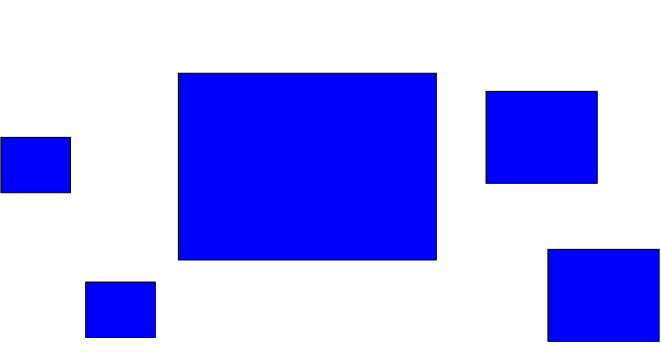
\includegraphics[width=.25\textwidth]{simetria-ninguna}}
      & \fbox{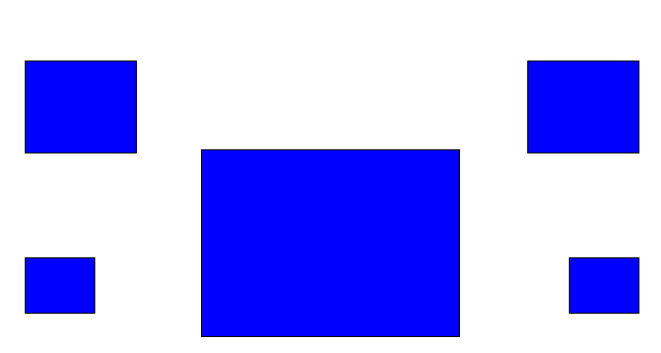
\includegraphics[width=.25\textwidth]{simetria-vertical}}
      & \fbox{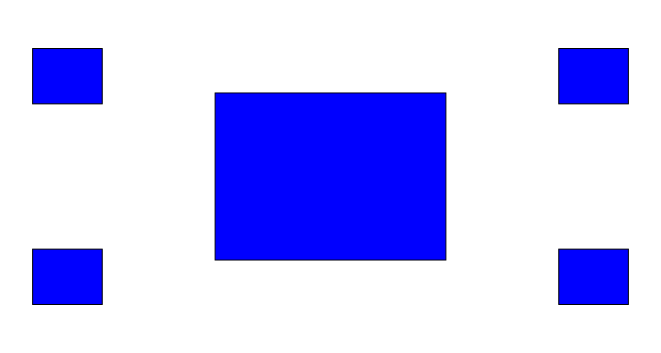
\includegraphics[width=.25\textwidth]{simetria-ambos}} \\[1ex]
      Sin simetría & Horizontal & Horizontal y vertical
    \end{tabular}
  \end{center}

\end{frame}

\begin{frame}{Esquemas de colores (I)}

  \begin{block}{¿Cómo los elijo?}
    \begin{itemize}
    \item Para mayor legibilidad, hay que maximizar el contraste: lo
      ideal es usar letra oscura sobre fondo claro
    \item Tienen que ser colores <<compatibles>>: no conviene mezclar
      colores calientes con fríos, excepto para resaltar algo
    \item \url{http://colorschemedesigner.com} $\rightarrow$
      <<complement>> y color principal azul: ¿qué os sale?
    \end{itemize}
  \end{block}

  \begin{block}{Diferencias en percepción de colores entre personas}
    \begin{itemize}
    \item 8\% de los hombres y $0.4$\% de las mujeres tienen
      \href{http://en.wikipedia.org/wiki/Color_blindness\#cite_note-Howard_Hughes_Medical_Institute-28}{algún
        problema} distinguiendo colores
    \item Wikipedia tiene
      \href{http://en.wikipedia.org/wiki/Category:Articles_with_images_not_understandable_by_color_blind_users\#Tips_for_editors}{indicaciones},
      y hay simuladores de pantalla completa como
      \href{http://colororacle.org/}{ColorOracle}
    \end{itemize}
  \end{block}

\end{frame}

\begin{frame}{Esquemas de colores (II)}

  \begin{block}{Importancia del medio}
    \begin{itemize}
    \item Cada pantalla, monitor, impresora o cañón representa los
      colores de forma distinta
    \item Además, el espacio de colores en monitores (RGB) es distinto
      al de las impresoras (CMYK, PMS)
    \item Los diseñadores gráficos profesionales calibran su monitor
      contra un perfil de color apropiado y elaboran materiales sobre
      CMYK o PMS, pero puede ser complejo y caro
    \item Una aproximación razonable es imprimir un borrador antes de
      mandarlo a la imprenta, para ver si los colores salen bien
    \end{itemize}
  \end{block}
  
\end{frame}

\begin{frame}{Texto: tamaño, fuentes y alineaciones}

  \begin{block}{Tamaños de letra}
    \begin{itemize}
    \item Títulos legibles desde 4--6m y texto desde 2m
    \item Los títulos y subtítulos deben resaltar sobre el texto normal
    \item En el ordenador, probad a leerlo al 33\% o 25\%
    \item Imprimidlo a A4: el texto debe ser legible
    \end{itemize}
  \end{block}

  \begin{block}{Tipos de letra}
    \begin{itemize}
    \item Hay dos familias fundamentales: sans (texto en pantalla) y
      \textrm{serif} (texto en impresión)
    \item Además, hay variantes proporcionales (texto normal) y
      \texttt{monoespaciadas} (código o salida de un programa)
    \end{itemize}
  \end{block}

  \begin{block}{Alineación justificada}
    Especialmente mala en pósters si se hace mal (no usáis \LaTeX).
  \end{block}

\end{frame}

\begin{frame}{Formatos de imágenes (I)}
  \begin{center}
    \includegraphics[width=.9\textwidth,height=.8\textheight,keepaspectratio]{Bitmap_VS_SVG}

    Comparación entre mapas de bits y gráficos vectoriales
    (\href{http://en.wikipedia.org/wiki/File:Bitmap_VS_SVG.svg}{Wikipedia},
    <<Bitmap VS SVG>>, CC-BY-SA 2.5)
  \end{center}
\end{frame}

\begin{frame}{Formatos de imágenes (II)}
  \framesubtitle{Fotos: JPEG, gráficas: SVG (PNG de alta resolución si no hay más remedio)}

  \begin{block}{Mapas de bitmaps: JPEG, PNG, BMP, GIF, PCX...}
    \begin{itemize}
    \item Imagen = matriz de \emph{pixels}
    \item Se <<pixelan>> al ampliarlas: es mejor trabajar con imágenes
      grandes y luego reducirlas sobre la marcha
    \item JPEG: formato <<con pérdidas>>, para fotografías
    \item PNG: formato <<sin pérdidas>>, para gráficas y dibujos
      lineales
    \item Al escanear, hay que usar 150ppp como mínimo
    \end{itemize}
  \end{block}

  \begin{block}{Vectoriales: SVG, AI, EPS...}
    \begin{itemize}
    \item Imagen = secuencia de instrucciones de dibujado
    \item Pueden escalarse libremente sin problemas
    \item SVG: estándar abierto, textual, leído por muchos nav.\ Web
    \end{itemize}
  \end{block}
\end{frame}

\begin{frame}{Gráficas utilizadas: mediciones puntuales}

  \begin{itemize}
  \item Pensad bien en el tipo de medición a representar
  \item Etiquetad ejes e indicad unidades
  \item Evitad efectos 3D, sombras y cosas que no añaden información
  \end{itemize}

  \vfill

  \begin{center}
    \begin{tabular}{*{2}{>{\centering\arraybackslash}p{.45\textwidth}}}
      \begin{tikzpicture}
        \begin{axis}[width=.4\textwidth, enlarge x limits=true, xlabel=$x$, ylabel={$f(x)$ (unidad)}]
          \addplot+ coordinates {(0,1) (1,2) (2,3) (4,8) (5,10) (6,20) (7,30) (8,40)};
        \end{axis}
      \end{tikzpicture}
      &
      \begin{tikzpicture}
        \begin{axis}[width=.4\textwidth, symbolic x coords={A,B,C}, enlarge x limits=true, xlabel=Categorías, ylabel=Resultados (unidad)]
          \addplot[fill=blue,ybar] coordinates {(A,1) (B,2) (C,3)};
        \end{axis}
      \end{tikzpicture} \\
      Variable dependiente continua o discreta con muchos valores &
      Variable discreta o categórica
    \end{tabular}
  \end{center}

\end{frame}

\begin{frame}{Gráficas utilizadas: medias y medianas}
  \begin{center}
    \begin{tabular}{*{2}{>{\centering\arraybackslash}p{.45\textwidth}}}
      \begin{tikzpicture}
        \begin{axis}[
          width=.4\textwidth,
          symbolic x coords={A,B,C},
          only marks,
          enlarge x limits=true,
          xlabel=Categorías,
          ylabel=Medias y límites (unidad)
          ]
          \addplot+[draw=black, fill=white, error bars/.cd, y dir=plus, y explicit]
            coordinates {
              (A, 1) +- (0, 0.5)
              (B, 2) +- (0, 0.7)
              (C, 0.7) +- (0, 1.2)
            }; 
          \addplot[draw=black, fill=white, error bars/.cd, y dir=minus, y explicit]
            coordinates {
              (A, 1) +- (0, 0.8)
              (B, 2) +- (0, 1)
              (C, 0.7) +- (0, 0.6)
            };
        \end{axis}
      \end{tikzpicture}
      &
      \begin{tikzpicture}
        \begin{axis} [
          width=.4\textwidth,
          xtick=data,
          symbolic x coords={A, B, C},
          enlarge x limits={0.2},
          xlabel=Categorías,
          ylabel=Resultados (unidad)
          ]
          \addplot [box plot median] table {testdata.dat};
          \addplot [box plot box] table {testdata.dat};
          \addplot [box plot top whisker] table {testdata.dat};
          \addplot [box plot bottom whisker] table {testdata.dat};
        \end{axis}
      \end{tikzpicture} \\
      Medias (distribución normal) & Medianas (otra distribución)
    \end{tabular}

    \vfill

    Si usáis barras de error como en la izquierda, no olvidéis
    \href{http://betterposters.blogspot.com/2012/01/error-bars.html}{indicar}
    qué tipo de <<error>> es: ¿mínimo y máximo? ¿Desviación típica?
    ¿Intervalo de confianza?
  \end{center}

\end{frame}

\begin{frame}{Códigos QR}

  \begin{block}{Utilidad}
    \begin{itemize}
    \item Pueden imprimirse de forma normal
    \item Pueden contener una tarjeta de visita o un enlace a una web
    \item Los lectores con \emph{smartphones} puede que tengan
      curiosidad
    \item Hay generadores de códigos QR
      \href{http://zxing.appspot.com/generator/}{gratuitos}
    \end{itemize}
  \end{block}

  \begin{center}
    \includegraphics[height=.4\textheight]{qr_code}

    ¿A dónde va este código QR?
  \end{center}

\end{frame}

\subsection[Software]{Software utilizable}

\begin{frame}{Antes de abrir el programa}

  \begin{block}{Preguntas para la organización}
    \begin{itemize}
    \item ¿Qué formatos físicos se admiten?
    \item ¿Hay algo que deba ponerse en todas las transparencias?
    \end{itemize}
  \end{block}

  \begin{block}{Preguntas para la imprenta}
    \begin{itemize}
    \item ¿Qué formatos de fichero aceptan? $\rightarrow$ PDF es ideal
    \item ¿Hay alguna limitación de colores o tamaño en el proceso?
    \end{itemize}
  \end{block}
  
\end{frame}

\begin{frame}{De elaboración de presentaciones}

  \begin{block}{Ejemplos}
    \begin{itemize}
    \item LibreOffice Impress (libre)
    \item Microsoft PowerPoint, Keynote (privativos)
    \end{itemize}
  \end{block}

  \begin{block}{Ventajas}
    \begin{itemize}
    \item Fáciles de usar y conocidos
    \item Normalmente ya tenemos uno instalado
    \end{itemize}
  \end{block}

  \begin{block}{Desventajas}
    \begin{itemize}
    \item Dan menos facilidades a la hora de colocar elementos
    \item Tienen menos opciones para el formato
    \item Los resultados pueden variar mucho entre ordenadores
    \item Normalmente es mejor usar otro tipo de software
    \end{itemize}
  \end{block}

\end{frame}

\begin{frame}{De dibujo}

  \begin{block}{Ejemplos}
    \begin{itemize}
    \item Inkscape, Krita o LibreOffice Draw (libres)
    \item OmniGraffle o Adobe Illustrator (privativos)
    \end{itemize}
  \end{block}

  \begin{block}{Ventajas}
    \begin{itemize}
    \item Relativamente fáciles de usar
    \item Más funcionalidad que los de elaboración de presentaciones:
      alineación de elementos, formas personalizadas, máscaras,
      conexión de elementos de diagramas, texto sobre rutas, etc.
    \end{itemize}
  \end{block}

  \begin{block}{Desventajas}
    \begin{itemize}
    \item Aún nos obligan a colocarlo y distribuirlo todo a mano
    \end{itemize}
  \end{block}
  
\end{frame}

\begin{frame}{De maquetación}

  \begin{block}{Ejemplos}
    \begin{itemize}
    \item Scribus (libre)
    \item Microsoft Publisher (básico, privativo)
    \item Adobe InDesign/FrameMaker (privativo)
    \end{itemize}
  \end{block}

  \begin{block}{Ventajas}
    \begin{itemize}
    \item Mayor funcionalidad y nivel de control
    \item Permiten controlar el flujo del texto y su división en
      columnas y otros elementos, el espaciado, etc.
    \end{itemize}
  \end{block}

  \begin{block}{Desventajas}
    \begin{itemize}
    \item Curva elevada de aprendizaje
    \item Alto coste de las soluciones propietarias
    \end{itemize}
  \end{block}

\end{frame}

\begin{frame}{Otras soluciones}

  \begin{block}{PosterGenius: fácil, pero restrictivo}
    \begin{itemize}
    \item Prácticas comunes y plantillas prefabricadas para pósters
    \item Obliga a ir por columnas y no permite gráficos vectoriales
    \end{itemize}
  \end{block}

  \begin{block}{\LaTeX, por supuesto \Smiley}
    \begin{itemize}
    \item Curva de aprendizaje pronunciada, pero merece la pena
    \item Se puede incrustar código \LaTeX{} en otras herramientas
      (p. ej. \href{http://blogs.ethz.ch/kowalski/2011/10/05/inkscape-and-latex/}{Inkscape}
      o
      \href{http://www.mostlymaths.net/2010/11/mathematics-poster-dropbox-scribus-and.html}{Scribus})
      para fórmulas y texto de alta calidad
    \item Se puede usar de forma
      \href{http://www.tex.ac.uk/cgi-bin/texfaq2html?label=poster}{independiente}
      para hacer pósters mediante
      \href{http://nxg.me.uk/docs/posters/}{a0poster}, \href{http://www.brian-amberg.de/uni/poster/}{baposter} o
      \href{http://www-i6.informatik.rwth-aachen.de/~dreuw/latexbeamerposter.php}{beamerposter},
      por ejemplo
    \end{itemize}
  \end{block}

  \begin{block}{Software de edición de fotos}
    \begin{itemize}
    \item GIMP (libre) o Adobe Photoshop (privativo)
    \item No recomendados
    \end{itemize}
  \end{block}
  
\end{frame}

\subsection{Impresión y montaje}

\begin{frame}{Tamaños habituales}
  \begin{columns}
    \column{.5\textwidth}

    \begin{center}
      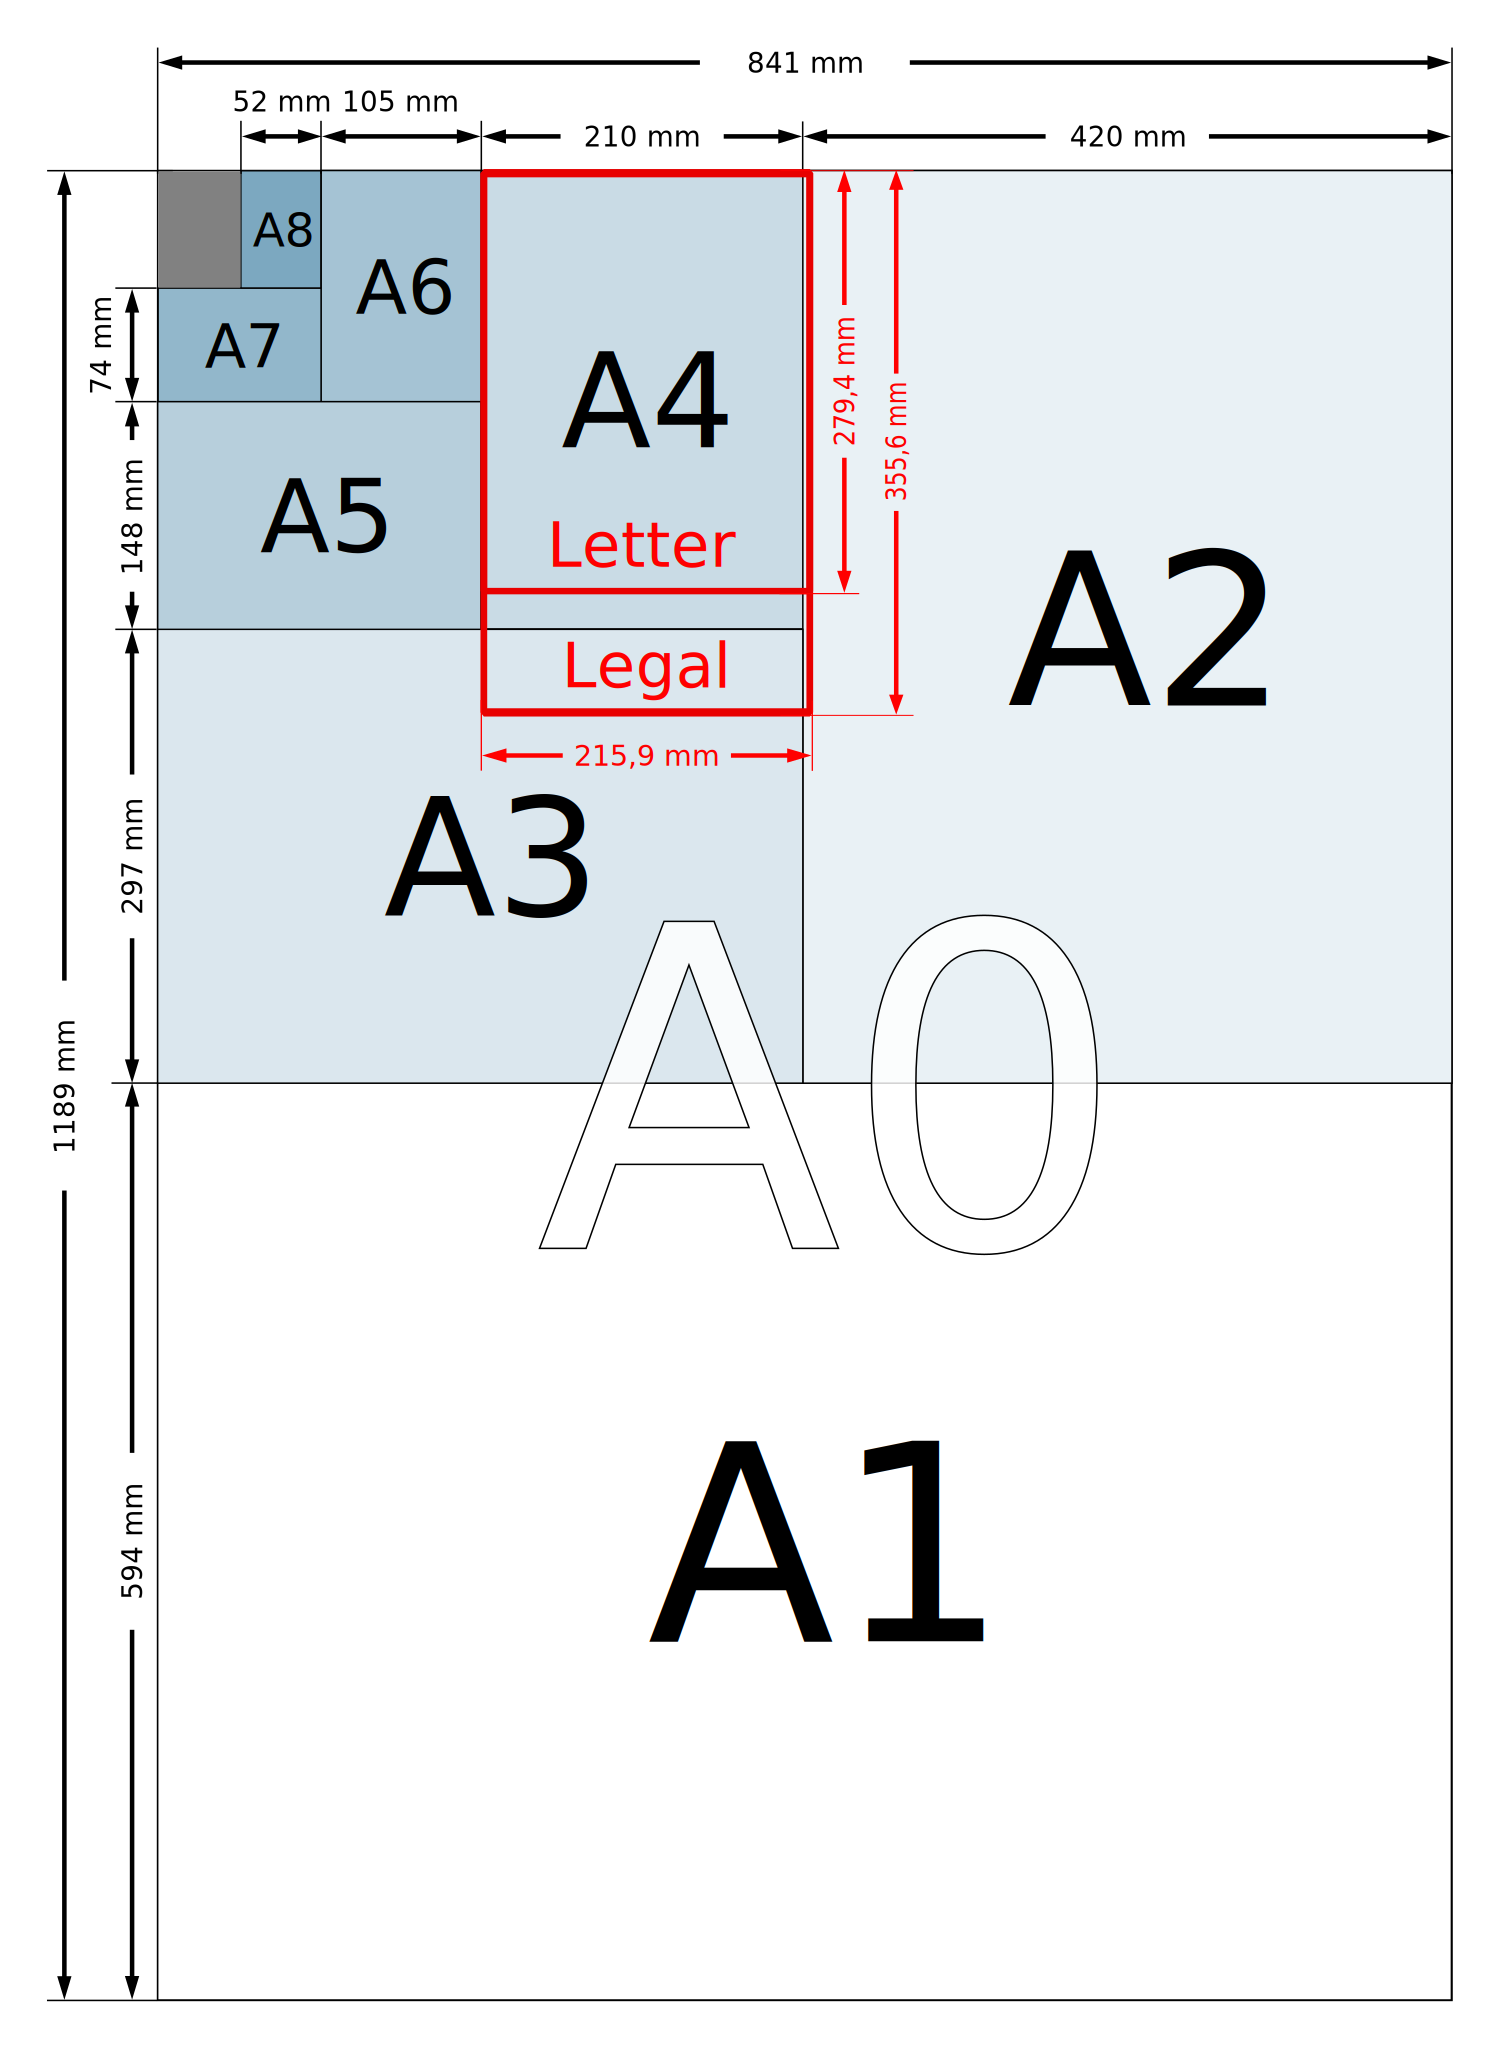
\includegraphics[width=\textwidth,height=.7\textheight,keepaspectratio]{A_size_illustration2_with_letter_and_legal}

      Tamaños ISO 216 A (\href{http://en.wikipedia.org/wiki/File:A_size_illustration2.svg}{Wikipedia}, <<ISO 216>>, CC-BY-SA 3.0)
    \end{center}

    \column{.5\textwidth}
    \begin{itemize}
    \item A0 (841mm $\times$ 1189mm) es popular en Europa: ocupa 4 A4
      de alto y 4 A4 de ancho
    \item En eventos fuera de Europa, puede que se usen medidas
      imperiales, como 2 $\times$ 4 pies, por ejemplo
    \item Los formatos en retrato sugieren usar disposiciones en
      filas, y en apaisado es mejor ir en columnas
    \end{itemize}
  \end{columns}
\end{frame}

\begin{frame}{Materiales habituales}
  \hypersetup{colorlinks,linkcolor=blue}

  \begin{block}{Papel: barato, mejor impresión}
    \begin{itemize}
    \item Antes era común pegar fotos y texto sobre una cartulina,
      pero hoy en día lo normal es mandar a imprimir un cartel
    \item Si pensabais imprimir 16 A4 y juntarlos con cinta
      adhesiva... \href{http://www.flickr.com/photos/damienclauzel/4465767871/}{pensadlo
        bien} (bueno, eso era un borrador)
    \item Tened en cuenta el gramaje del papel: un papel de mayor
      calidad aguantará mejor el transporte y puede ser reutilizable
    \item Laminar el papel es buena idea, pero lo hará menos flexible
      y más difícil de transportar (¡cuidado al coger el vuelo!)
    \end{itemize}
  \end{block}

  \begin{block}{Lona o vinilo: algo más cara, pero mucho más resistente}
    \begin{itemize}
    \item Es mucho más resistente y flexible, y no excesivamente cara
    \item Cuidado con pósters con dibujos lineales: las líneas
      tienden a correrse si no se seca bien en la imprenta
    \end{itemize}
  \end{block}

\end{frame}

\begin{frame}{Montaje de un póster}

  \begin{block}{Sobre superficie: cinta adhesiva normal}
    Resulta poco estética, al verse desde fuera. Si el póster es de
    papel, puede retirar parte de la tinta al quitarse.
  \end{block}

  \begin{block}{Sobre superficie: cinta adhesiva de doble cara}
    No se ve desde fuera y no retirará nada visible al quitarse. De
    todos modos, si es de papel, cuidado al quitarlo: se podría
    rasgar.
  \end{block}

  \begin{block}{Montado a nivel de suelo: lona y ojales}
    Si tiene que ir montado a nivel de suelo, normalmente se
    enganchará a un armazón, por lo que necesitaréis un cartel de lona
    o vinilo con los
    \href{http://www.printcolorweb.com/spa/item/index.html?msgOrigen=9\&msgValor=58\&CODART=lona}{ojales
      apropiados}.
  \end{block}

\end{frame}

\section{Defensa}

\begin{frame}{Recomendaciones para el día de la sesión (I)}

  \begin{block}{Cuidar el aspecto físico y lenguaje corporal}
    \begin{itemize}
    \item Evidentemente, hay que venir descansado, limpio y arreglado
    \item Ir en chaqueta o no depende de la cultura de vuestra
      especialidad: en informática basta con ir bien vestido
    \item Curiosidad: si la ropa está conjuntada con el póster,
      \href{http://www.cmaj.ca/content/169/12/1291.full}{mejor}
    \item El lenguaje corporal es importante: cruzar los brazos o
      meter las manos en los bolsillos crea una barrera invisible
    \end{itemize}
  \end{block}

  \begin{block}{Colocarse y atraer al público}
    \begin{itemize}
    \item Si no hay sitios designados para cada póster, buscar el más
      cercano al café o por el que pase todo el mundo
    \item No es mala idea atraer al público con detalles sencillos, si
      los tenemos: bolígrafos, CD, alguna muestra relacionada con el
      tema de investigación
    \end{itemize}
  \end{block}

\end{frame}

\begin{frame}{Recomendaciones para el día de la sesión (II)}

  \begin{block}{Atender a los visitantes}
    \begin{itemize}
    \item Si sólo están interesados en leer, dejarles tranquilos
    \item Si preguntan, \structure{nunca} leer el póster en voz alta:
      \begin{enumerate}
      \item Resumir en una frase lo que se ha hecho
      \item Ir describiendo más en detalle señalando figuras
      \item Responder a preguntas sobre la marcha
      \item Si viene alguien más, que espere
      \end{enumerate}
    \item Vigilad el lenguaje corporal de la otra persona
    \end{itemize}
  \end{block}

  \begin{block}{Obtener contactos}
    \begin{itemize}
    \item Es buena idea traer tarjetas de visita, folletos o copias
      impresas en A4 de vuestro póster/artículo, si podéis
    \item Si os deja la organización, otra opción es poner una cajita
      al lado del póster y que los interesados cojan una tarjeta o
      folleto
    \end{itemize}
  \end{block}

\end{frame}

\section[Ejemplos]{Ejemplos de pósters}
\label{sec:posters}

\begin{frame}{Ejemplos}
  \begin{center}

    \vspace{\stretch{3}}

    {\Large Veamos algunos ejemplos.}

    \vspace{\stretch{3}}

    {\large \url{http://www.flickr.com/groups/postersessions/}}

    \vspace{\stretch{1}}

    {\large \url{http://f1000.com/posters}}
  \end{center}
\end{frame}

\appendix

\begin{frame}{Para aprender más}
  \framesubtitle{Cuidado: no todos los ejemplos son buenos}

  \begin{thebibliography}{10}
    \beamertemplatearticlebibitems
    \bibitem{x} Zen Faulkes.
      \newblock Blog <<Better Posters>>.
      \newblock {\small\url{http://betterposters.blogspot.com}}

    \bibitem{y} Purrington, C.B.
      \newblock Designing conference posters.
      \newblock {\small\url{http://colinpurrington.com/tips/academic/posterdesign}}

    \bibitem{x} Colorado State University.
      \newblock Writing Guide: Poster Sessions.
      \newblock {\small\url{http://writing.colostate.edu/guides/speaking/poster/}}
  \end{thebibliography}
\end{frame}

\begin{frame}{Fin de la presentación}
  \begin{center}

    \vspace{\stretch{3}}

    {\Huge ¡Gracias!}

    \vspace{\stretch{3}}

    {\Large
      \href{mailto:antonio.garciadominguez@uca.es}{antonio.garciadominguez@uca.es}

      \vspace{\stretch{1}}

      Twitter: \href{http://twitter.com/antoniogado}{@antoniogado}}
  \end{center}
\end{frame}

\end{document}
